% Author: Rasmus Pank Roulund
% Inspired by figure in:
% Howells, Peter og Bain, Keith (2007). Financial markets and
% institutions. 5. udg. Essex: Pearson Education.
\documentclass{minimal}
\usepackage{tikz}
\usepackage{verbatim}

\begin{comment}
:Title: Borrowers and lenders

An illustration inspired by Figure 1.1 in Howells, Peter og Bain, Keith (2007), 
Financial markets and institutions. 5th ed. Essex: Pearson Education.

\end{comment}

\usetikzlibrary{arrows,positioning} 
\tikzset{
    %Define standard arrow tip
    >=stealth',
    %Define style for boxes
    punkt/.style={
           rectangle,
           rounded corners,
           draw=black, very thick,
           text width=6.5em,
           minimum height=2em,
           text centered},
    % Define arrow style
    pil/.style={
           ->,
           thick,
           shorten <=2pt,
           shorten >=2pt,}
}

\begin{document}

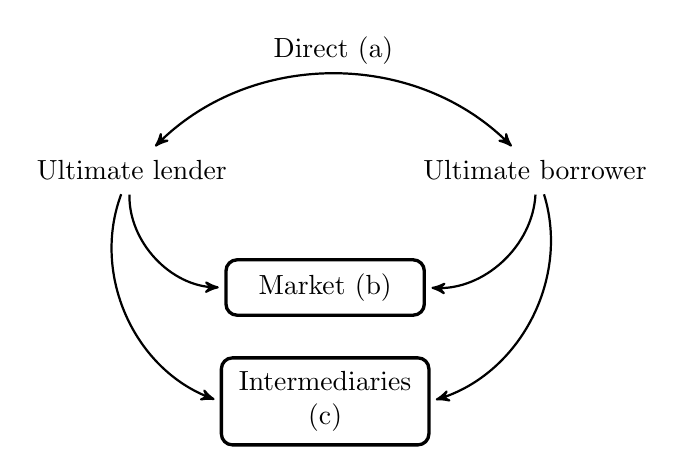
\begin{tikzpicture}[node distance=1cm, auto,]
 %nodes
 \node[punkt] (market) {Market (b)};
 \node[punkt, inner sep=5pt,below=0.5cm of market]
 (formidler) {Intermediaries (c)};
 % We make a dummy figure to make everything look nice.
 \node[above=of market] (dummy) {};
 \node[right=of dummy] (t) {Ultimate borrower}
   edge[pil,bend left=45] (market.east) % edges are used to connect two nodes
   edge[pil, bend left=45] (formidler.east); % .east since we want
                                             % consistent style
 \node[left=of dummy] (g) {Ultimate lender}
   edge[pil, bend right=45] (market.west)
   edge[pil, bend right=45] (formidler.west)
   edge[pil,<->, bend left=45] node[auto] {Direct (a)} (t);
\end{tikzpicture}

\vspace{1em}
\emph{Inspired by figure 1.1 in ``Financial Markets and Institutions'' 5E
  by Howells and Bain.}
\end{document}

%%% Local Variables:
%%% mode: latex
%%% TeX-master: t
%%% End:
